\documentclass[12pt, a4paper]{article}

\usepackage{amsmath}
\usepackage{amsfonts}
\usepackage{graphicx}
\usepackage{pdfpages}
\usepackage[titletoc, title]{appendix}
\usepackage{hyperref}
\hypersetup{
    colorlinks=true,
    linkcolor=blue,
    filecolor=magenta,      
    urlcolor=cyan,
}


\def\vb{\boldsymbol{b}}
\def\vh{\boldsymbol{h}}
\def\vw{\boldsymbol{w}}
\def\vx{\boldsymbol{x}}
\def\vy{\boldsymbol{y}}
\def\vz{\boldsymbol{z}}
\def\v1{\boldsymbol{1}}

\def\vI{\boldsymbol{I}}
\def\vW{\boldsymbol{W}}
\def\vX{\boldsymbol{X}}
\def\vY{\boldsymbol{Y}}

\def\vtheta{\boldsymbol{\theta}}

\def\rmx{\mathrm{x}}

\def\vrmx{\boldsymbol{\mathrm{x}}}
\def\vrmy{\boldsymbol{\mathrm{y}}}
\def\vrmX{\boldsymbol{\mathrm{X}}}
\def\vrmY{\boldsymbol{\mathrm{Y}}}

\def\E{\mathbb{E}}
\def\X{\mathbb{X}}
\def\R{\mathbb{R}}

\def\st{\textit{s.t.}}

\DeclareMathOperator*{\relu}{ReLU}
\DeclareMathOperator*{\argmax}{arg\,max}
\DeclareMathOperator*{\argmin}{arg\,min}
\DeclareMathOperator*{\softmax}{softmax}

\newcommand{\egvx}[1]{\boldsymbol{x}^{(#1)}}
\newcommand{\egvy}[1]{\boldsymbol{y}^{(#1)}}
\newcommand{\egx}[1]{x^{(#1)}}
\newcommand{\egy}[1]{y^{(#1)}}
\newcommand{\eghy}[1]{\hat{y}^{(#1)}}

\newcommand{\expect}[3]{\mathbb{E}_{#1 \sim #2} \left[ #3 \right]}
\newcommand{\dkl}[2]{D_{\mathrm{KL}}(#1 \Vert #2)}
\newcommand{\condiP}[3]{P(#1 \mid #2;#3)}
\newcommand{\condip}[3]{p(#1 \mid #2;#3)}
\newcommand{\ND}[3]{\mathcal{N}(#1;#2,#3)}

\newcommand{\dx}[1]{\frac{\mathrm{d}}{\mathrm{d}x} #1}
\newcommand{\pard}[2]{\frac{\partial #1}{\partial #2}}


\title{Back Propagation}
\author{CHEN Si}
\date{}


\begin{document} 


\maketitle
\tableofcontents


\section{Motivation}
\begin{itemize}
    \item The back-propagation algorithm is designed to reduce the number of common subexpressions without regard to memory.
    \begin{itemize}
        \item Storing the subexpressions is preferable because of its reduced runtime.
        \item Computing twice the subexpressions is useful when memory is limited.
    \end{itemize}
\end{itemize}


\section{Chain Rule of Calculus}
\begin{itemize}
    \item The back-propagation algorithm consists of performing such a Jacobian-gradient product for each operation in the graph.
    \item We could imagine flattening each tensor into a vector before we run back-propagation.
\end{itemize}

\paragraph{For vectors}
Suppose that $\vx \in \R^m,\ \vy \in \R^n,\ g: \R^m \to \R^n,\ f: \R^n \to \R$.
If $\vy = g(\vx),\ z = f(\vy)$, then
\[
    \pard{z}{x_i} = \sum_j \pard{z}{y_j} \pard{y_j}{x_i}
\]
In vector notation, equivalently written as
\[
    \nabla_{\vx} z = \left( \pard{\vy}{\vx} \right)^\top \nabla_{\vy} z
\]
, where $\pard{\vy}{\vx} \in R^{n\times m}$ is the Jacobian matrix of $g$, \st $\left( \pard{\vy}{\vx} \right)_{i,j} = \pard{}{x_j} g(\vx)_i$.

\paragraph{For tensors}
If $\vrmY = g(\vrmX),\ z = f(\vrmY)$, then 
\[
    \nabla_{\vrmX}z = \sum_j (\nabla_{\vrmX}Y_j) \pard{z}{Y_j}
\]
, where $j$ represents the complete tuple of indices of tensor $\vrmY$ and $(\nabla_{\vrmX}z)_i = \pard{z}{X_i}$.


\section{Simple Scalar Version}

\subsection{Forward Computation}
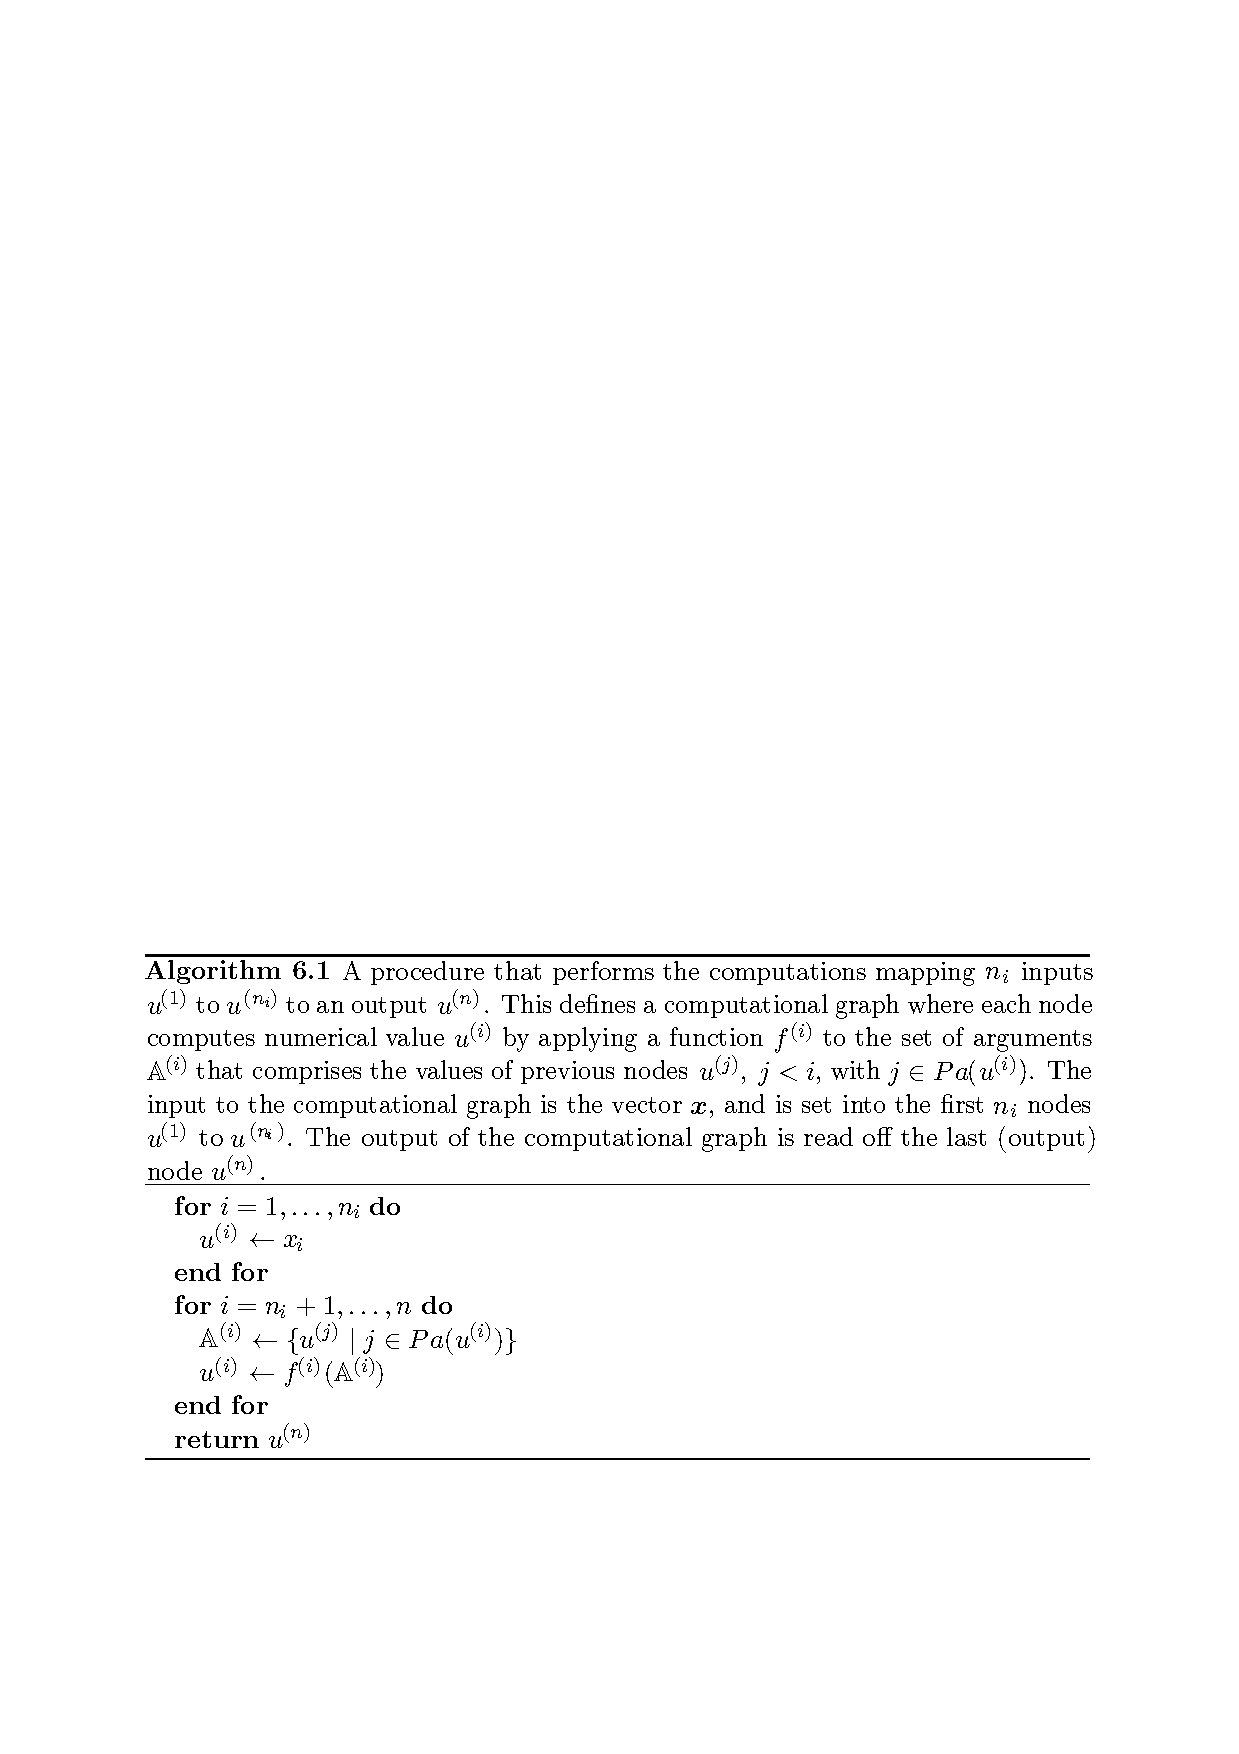
\includegraphics[width=\textwidth]{../imgs/Forward_Computation.pdf}

\subsection{Back Propagation}
\includegraphics[width=\textwidth]{../imgs/Back_propagation.pdf}


\section{MLP Version}
\subsection{Forward Computation}
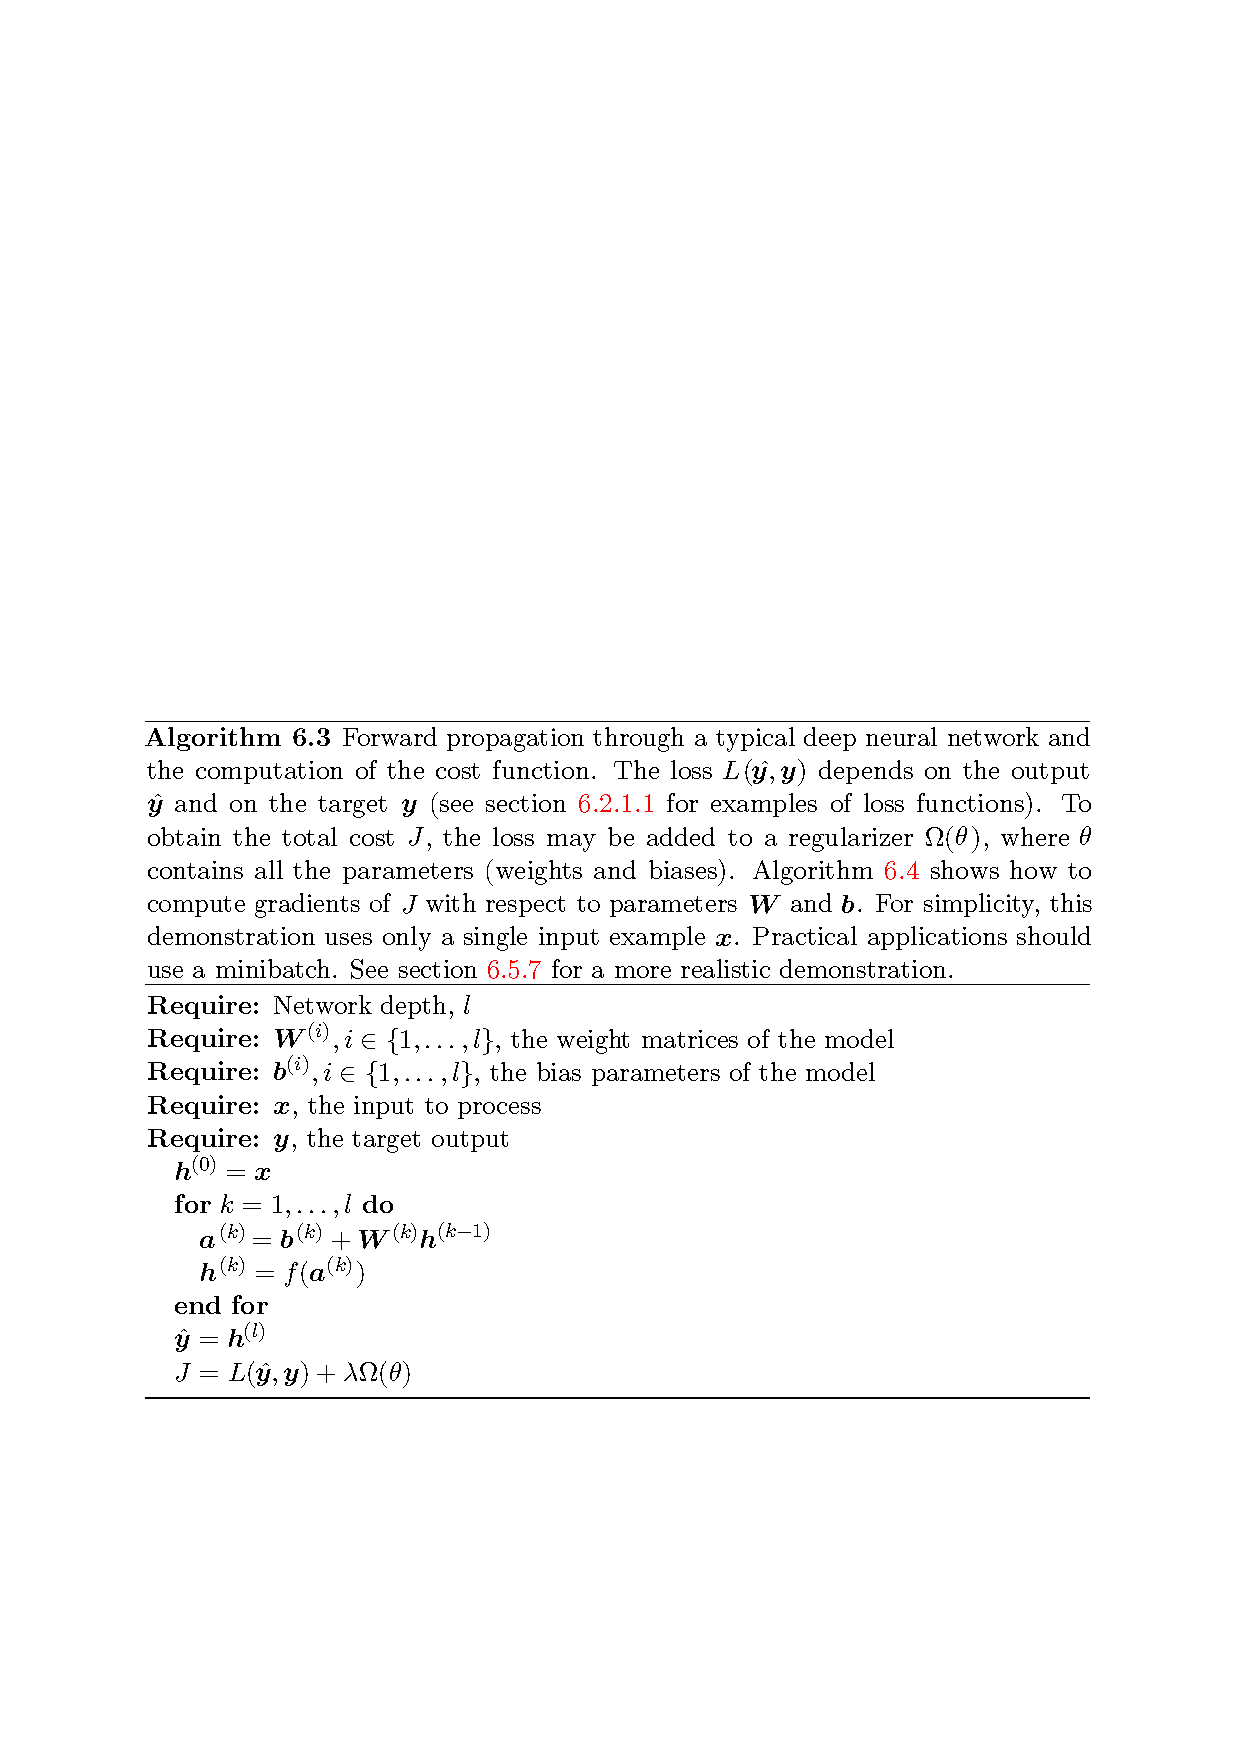
\includegraphics[width=\textwidth]{../imgs/Forward_Computation_of_MLP.pdf}
\subsection{Back Propagation}
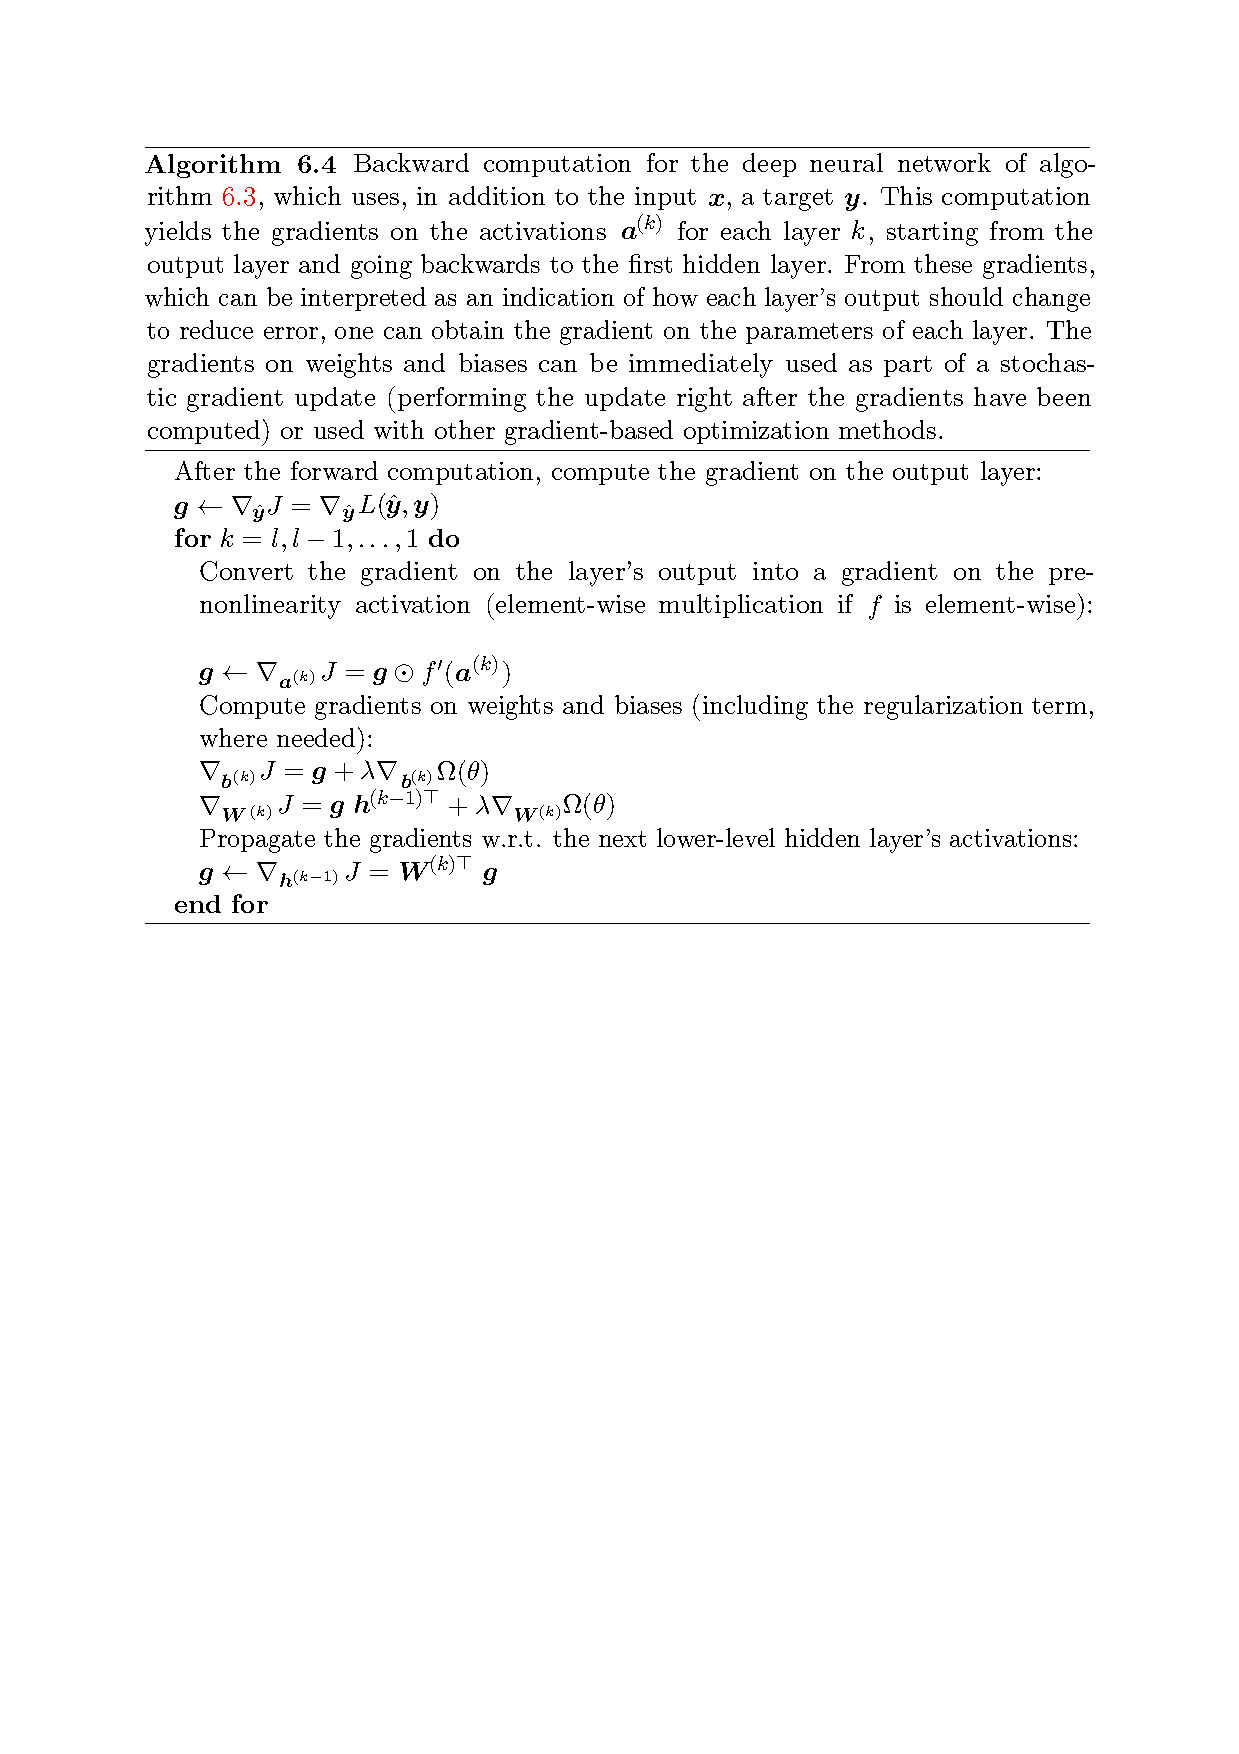
\includegraphics[width=\textwidth]{../imgs/Back_Propagation_of_MLP.pdf}


\end{document}